\documentclass[10pt]{beamer}

\usetheme{m}

\usepackage{booktabs}
\usepackage[scale=2]{ccicons}

\usepackage[T1]{fontenc}
\usepackage[brazil]{babel}
%\usepackage[latin1]{inputenc}

\usepackage{pgfplots}
\usepgfplotslibrary{dateplot}

\title{Aplicando o Arcabouço OpenTuner em Jogos Digitais}
\date{\today}
\author{Renan Teruo Carneiro e Vitor Cerqueira Santos\\
	Orientador: Prof. Dr. Alfredo Goldman\\
    Co-orientador: Pedro Bruel}
\institute{Instituto de Matemática e Estatística}
% \titlegraphic{\hfill\includegraphics[height=1.5cm]{logo/logo}}

\begin{document}

\maketitle

%\begin{frame}
%  \frametitle{Table of Contents}
%  \setbeamertemplate{section in toc}[sections numbered]
%  \tableofcontents[hideallsubsections]
%\end{frame}

\section{Introdução}

\begin{frame}[fragile]
	\frametitle{Otimização de Parâmetros}
	  \begin{itemize}[<+- | alert@+>]
	  	\item Aplicação com várias configurações
	  	\item Problema: Encontrar melhor conjunto de configurações
	  	\item Autotuning is hooray
	  	\item OpenTuner is Hooray
	  \end{itemize}
\end{frame}

\begin{frame}{OpenTuner}
	Framework para Autotuning\pause\\
	Buscas marotas\pause\\
	Exploitation x Exploration\pause\\
	Is no paralelismo for shame
\end{frame}
%
%\begin{frame}[fragile]
%  \frametitle{Ajuste Fino}
%	  Enter the Autotuning!
%	  \pause
%	  \begin{itemize}[<+- | alert@+>]
%	  	\item Automatiza esse processo:
%	  	\item   Chuta uma configuração
%	  	\item   Vê o resultado
%	  	\item   Chuta outra configuração baseado nisso
%	  \end{itemize} 
%  %TODO: Autotuning
%  
%\end{frame}
%
%\begin{frame}[fragile]
%	\frametitle{Ajuste Fino}
%	Imagem goes here? Suplanta slide anterior?
%\end{frame}
%
%\begin{frame}[fragile]
%	\frametitle{Ajuste Fino}
%	  \begin{itemize}[<+- | alert@+>]
%	  	\item Geralmente feito do zero
%	  	\item Pessoal tem que manjar não só o programa, mas também buscas
%	  	\item Demora pra fazer
%	  	\item \begin{verbatim}= (\end{verbatim}
%	\end{itemize}
%\end{frame}



%\begin{frame}[fragile]
%  \frametitle{OpenTuner}
%      OpenTuner!
%      \pause
%	  \begin{itemize}[<+- | alert@+>]
%		\item Já tem técnicas prontas
%		\item Só precisa passar o que rodar e os parâmetros
%		\item Não está pronto
%		\item KEDE PARALELISMO AAAAAAAAAAAAAA \begin{verbatim} >=(\end{verbatim}
%		
%	  \end{itemize}  
%\end{frame}

\section{Ideias}

\begin{frame}[fragile]
  \frametitle{Ideias}
	  \begin{itemize}
	  	\item Geradores de Mapa
	  	\item Inteligências Artificias
	  	\item SaltyBet
	  	\item Builds de RPG e skilltrees
	  \end{itemize}
\end{frame}

\begin{frame}{Ideias}
	OpenTTD!
	\pause
	Explicação do OpenTTD!
\end{frame}

\begin{frame}{OpenTTD}	
	\begin{itemize}	[<+- | alert@+>]
		\item Open Source
		\item IAs
		\item Trens! Parte mais importante!
	\end{itemize}
\end{frame}

\section{Experimentos}
\begin{frame}{Experimentos}
	Ver o que acontece mexendo nos custos do pathfinder de uma IA.\pause\\
	Para isso, escolhemos a ChooChoo, porque trens. Sem mais.
\end{frame}

\begin{frame}{Experimentos}
	\begin{figure}
\centering
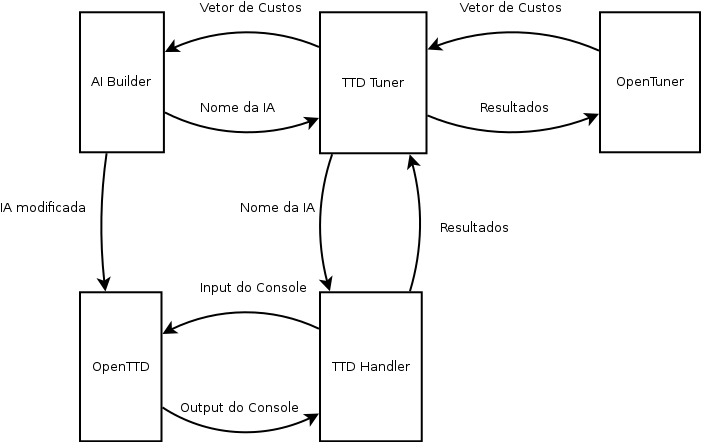
\includegraphics[width=1\linewidth]{Diagrama1}
\caption{Estrutura do tuner}
\label{fig:Diagrama1}
\end{figure}

\end{frame}
	
\begin{frame}{Experimentos}
	Esquemas altamente gambiarrísticos \pause\\
%	Builder <-> Tuner <-> Handler <-> OpenTTD <-> TRENS!!!!\pause\\
	OpenTTD compilado pra 0-player gotta go fast\pause\\
	Pode medir valor da empresa, dinheiro em caixa ou lucro no último quartil\pause\\
	Mede ao final de N anos, configurável\pause\\
	6 ou 8 IAs por iteração, pegando média\pause\\
	Demora \pause -> Servidores semiclandestinos\pause\\
	Altos crashes
\end{frame}

\section{Resultados e Conclusões}

\begin{frame}{Resultados e Conclusões}
	Funciona! \pause Kinda\pause\\
	OpenTuner conseguiu resultados sem saber como o programa funciona\pause \\
	Custos de pathfinder tem resultados reais. Who knew.\pause\\
	OpenTTD não foi feito pra ser automatizado, então usar o OpenTuner foi meio forçado\pause\\
	Talvez seja mais útil se um jogo for desenvolvido desde o começo com isso em mente
\end{frame}

\end{document}
